\chapter{Potencial Eléctrico} \label{chap:itv}
%% CAP 3 ITV. como se resuelve, resultados (solos, sin poros ni transporte). 
%% Comparar con formula cerrada?

En este capítulo se estudiará el potencial transmembrana generado en una célula por efecto de un pulso eléctrico, usando la ecuación \ref{eq:poisson} descrita en el capítulo anterior. Para eso se presentará el modelo computacional y los resultados serán estudiados. Se estudiará únicamente el potencial eléctrico en el dominio con su campo eléctrico, pero no se tendrá en cuenta la creación de poros en la membrana, los cuales pueden afectar la conductividad de la misma y modificar de esta manera el potencial eléctrico a través del tiempo. 

\section{Implementación}

Para resolver la ecuación \ref{eq:poisson} se utilizó el método de elementos finitos, llenando la matriz de rigidez según los conductividades y coordenadas de los elementos y el vector de masa según las condiciones de borde. La matriz de rigidez generada es simétrica definida positiva y con muy pocos elementos distintos de cero. Por estas razones es representada con una matriz esparsa y el sistema de ecuaciones se resuelve con el método de Cholesky. Una vez resuelto el sistema se obtiene el potencial eléctrico en cada nodo de la malla que representa el dominio. Dado que la creación de la matriz es uno de los pasos con mayor costo computacional, se utiliza \texttt{OpenMP} para llenar la matriz en paralelo, usando tantos threads como sean indicados en el archivo de entrada \texttt{input.in}.

Con los resultados obtenidos por el método de elementos finitos se calcula también el PTM en cada ángulo polar de la célula, comparando los potenciales externos con los internos, habiendo previamente identificado los nodos correspondientes al exterior e interior de cada ángulo discreto. También se calcula el campo eléctrico en el dominio como el gradiente del potencial eléctrico. Los resultados de potencial en el dominio, PTM y campo eléctrico se graban en archivos separados en formato \texttt{.csv}. 

La fórmula cerrada \ref{eq:cos} permitiría obtener con mayor facilidad los potenciales transmembrana sin resolver sistemas de ecuaciones, pero no es utilizada porque no sirve para obtener los potenciales en el resto del dominio, los cuales serán necesarios en capítulos posteriores y porque asume que la conductividad en la membrana es constante, lo cual no será asumido en el capítulo siguiente.

%TODO explicar mejor como se calcula el campo!!!

\newpage

\section{Resultados}
A continuación se presentan los resultados obtenidos de una simulación de una célula de 25\um de radio con dos electrodos que generan un campo eléctrico de 1200\vcm.\\

%\subsection*{Potencial en el dominio}

%\dobleimagen{itv/v-close}{itv-pote}{Potencial eléctrico en el dominio}{itv/campo-close}{itv-campo}{Campo eléctrico en el dominio}

\begin{wrapfigure}{r}{0.5\textwidth}
  \begin{center}
    %\includegraphics[width=0.48\textwidth]{gull}
    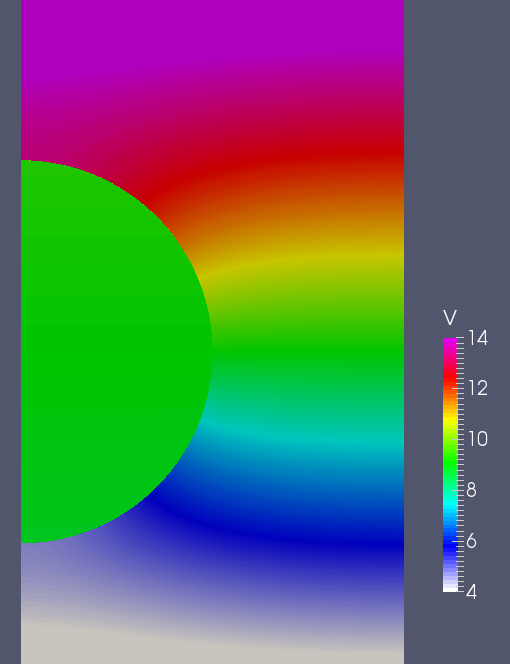
\includegraphics[width=0.48\textwidth]{itv/v-close}
  \end{center}
  \caption{Potencial eléctrico en el dominio}
  \label{fig:pote}
\end{wrapfigure}

Se observa en la figura \ref{fig:pote} que el potencial en el interior de la célula es constante y que la diferencia de potencial entre el exterior y el interior varía según la región de la superficie: en las regiones cercanas al ecuador de la célula la diferencia entre el interior y le exterior es casi nula, pero en los polos la diferencia se hace mayor. 

Las figuras \ref{fig:campo-r} y \ref{fig:campo-r-int} representan la componente horizontal del campo eléctrico en el dominio, con diferentes escalas que permiten observar las variaciones en el exterior e interior de la célula respectivamente. Los valores más altos se encuentran en exterior de la célula, con un campo en dirección positiva (hacia afuera de la célula) en el hemisferio polarizado, y negativa (hacia la célula) en el hemisferio depolarizado. Los valores en el interior de la célula son mucho menores, pero de signo opuesto al del exterior; con dirección hacia el exterior en el hemisferio depolarizado y hacia el interior en el hemisferio polarizado. Por último se nota que los valores más extremos se encuentran en la membrana, con signo opuesto al del exterior. 

En las figuras \ref{fig:campo-y} y \ref{fig:campo-y-int} se representa en cambio la componente vertical del campo eléctrico para el exterior e interior. En todos los casos el signo es negativo, por ser la dirección del campo hacia abajo. Los valores más extremos se encuentran en toda la membrana y en la zona extracelular, cerca del ecuador de la célula, mientras que ambos polos tienen los valores más cercanos a cero. En el interior de la célula el campo tiene valores con valor absoluto mucho menor, y al igual que en el exterior valores extremos cerca del ecuador y cercanos a cero en los polos.

%TODO EXPLICAR PORQUÉ EL CAMPO ES ASÍ EN TODOS LOS CASOS!!!!!

Por último en las figuras \ref{fig:campo} y \ref{fig:campo-int} se observa el módulo del campo eléctrico, teniendo en cuenta sus dos componentes, y se observan nuevamente los valores más extremos en la membrana y en zona del exterior cercana al ecuador.

En la figura \ref{fig:itv-vs-teo} se pueden comparar los resultados de PTM en función del ángulo polar obtenidos con la simulación de los indicados por la fórmula cerrada \ref{eq:cos}. Como puede observarse, los valores obtenidos con el método de elementos finitos son muy similares a los obtenidos con la fórmula cerrada, lo cual confirma el correcto funcionamiento de la simulación. 

\clearpage

\dobleimagen{itv/campo-r}{campo-r}{Componente horizontal del campo eléctrico}{itv/campo-r-int}{campo-r-int}{Componente horizontal del campo eléctrico en el interior de la célula}

\dobleimagen{itv/campo-y}{campo-y}{Componente vertical del campo eléctrico}{itv/campo-y-int}{campo-y-int}{Componente vertical del campo eléctrico en el interior de la célula}

\dobleimagen{itv/campo}{campo}{Módulo del campo eléctrico}{itv/campo-y-int}{campo-int}{Módulo del campo eléctrico en el interior de la célula}

%TODO unidad del campo???

%\dobleimagengrande{itv/itv-tita}{itv-tita}{PTM en función del  ángulo polar $\theta$\\ según simulación}{itv/itv-cos}{itv-cos}{PTM en función del  ángulo polar $\theta$\\ según fórmula cerrada}

\begin{figure}
	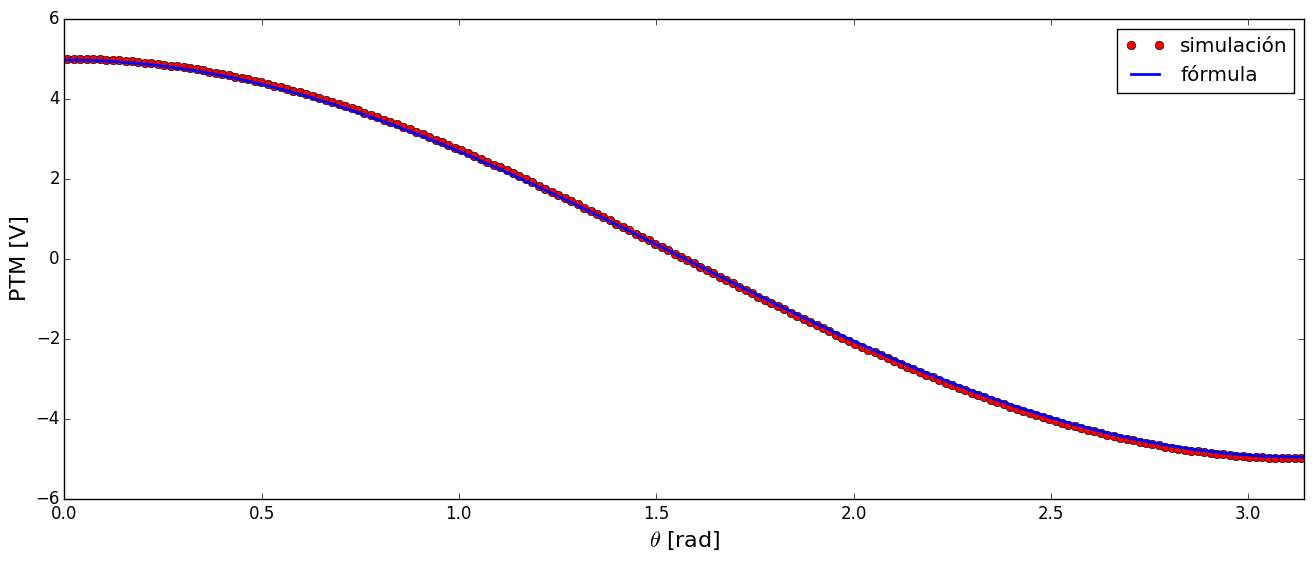
\includegraphics[width=1\textwidth]{itv/itv-vs-teo}
	\caption{PTM en función del ánglulo polar $\theta$ para E = 1600\vcm y $\alpha$ = 25\si{\micro\metre}. Resultados de la simulación y de la fórmula cerrada.}
	\label{fig:itv-vs-teo}
\end{figure}

\clearpage

También se realizaron simulaciones aplicando diferentes potenciales eléctricos y con células de diferentes radios. En la figura \ref{fig:itv-voltaje} se observa que el PTM aumenta linealmente al aumentar el campo eléctrico aplicado. También sucede lo mismo con el radio de la célula, como puede verse en la figura \ref{fig:itv-radio}. Nuevamente coinciden los resultados de las simulaciones con los de la fórmula cerrada \ref{eq:cos}, la cual indica que los valores de PTM son directamente proporcionales al campo eléctrico y el radio de la célula, y por lo tanto se necesitarán mayores valores de campo eléctrico para lograr un mismo potencial transmembrana cuanto más chica sea la célula.

\dobleimagengrande{itv/itv-voltaje}{itv-voltaje}{PTM en función del ángulo polar $\theta$ para\\ diferentes campos eléctricos aplicados}{itv/itv-radio}{itv-radio}{PTM en función del ángulo polar $\theta$ para\\ células de diferentes radios}
